\documentclass[newPxFont,noprogressbar,table]{beamer}
%\documentclass[newPxFont,sthlmFooter]{beamer}

%\documentclass[border=3mm,tikz,preview]{standalone}
%\usetikzlibrary{calc,backgrounds,positioning,fit}


\usetheme{sthlm}
%\usecolortheme{sthlmv42}

\setbeamertemplate{footline}[frame number]

%-=-=-=-=-=-=-=-=-=-=-=-=-=-=-=-=-=-=-=-=-=-=-=-=
%        LOADING PACKAGES
%-=-=-=-=-=-=-=-=-=-=-=-=-=-=-=-=-=-=-=-=-=-=-=-=
\usepackage[utf8]{inputenc}


% ADDED PACKAGES
%//////////////////////////////////////////////////////

\usepackage{helvet}
\renewcommand{\familydefault}{\sfdefault}
 
\usepackage[utf8]{inputenc}
%\usepackage[absolute,overlay]{textpos}
% Booktabs
\usepackage{booktabs}
\usepackage{multirow}
\usepackage{subfig}
% Algorithm package
\usepackage{algpseudocode} % Typesetting using the algorithmicx package
\renewcommand{\algorithmiccomment}[1]{\bgroup\hfill//~#1\egroup} % Algorithm comment

\usepackage{graphicx}
\usepackage{epstopdf}

\epstopdfDeclareGraphicsRule{.gif}{png}{.png}{convert gif:#1 png:\OutputFile}
\AppendGraphicsExtensions{.gif}

\setlength{\tabcolsep}{5pt}

% For floating point columns
\usepackage{etoolbox} 
\usepackage[tight-spacing=true]{siunitx}
\robustify\bfseries
% For bold cells using siunitx
\newcommand{\be}[2]{%
%	\multicolumn{1}{S[table-format=#1,
	\multicolumn{1}{>{\columncolor[HTML]{FFCE93}}S[table-format=#1,
		mode=text,
		text-rm=\fontseries{b}\selectfont
		]}{#2}}

% For bold cells using siunitx
\newcommand{\beUpperBound}[2]{%
	%	\multicolumn{1}{S[table-format=#1,
	\multicolumn{1}{>{\columncolor[HTML]{32CD32}}S[table-format=#1,
		mode=text,
		text-rm=\fontseries{b}\selectfont
		]}{#2}}


% Algorithm package
\usepackage{algorithm}
\usepackage{algpseudocode} % Typesetting using the algorithmicx package

\newenvironment{myitemize}
{ \begin{itemize}
		\setlength{\itemsep}{0pt}
		\setlength{\parskip}{0pt}
		\setlength{\parsep}{0pt}    
		\setlength\topsep{0pt}
		\setlength\partopsep{0pt}
}
{ \end{itemize}            }

\definecolor{sthlmOrange}{RGB}{154,51,36} % HEX #9A3324

%//////////////////////////////////////////////////////////////


\usepackage{todonotes}
\usepackage{adjustbox}

\setbeamertemplate{bibliography item}{\insertbiblabel}

%//////////////////////////////////////////////////////


%-=-=-=-=-=-=-=-=-=-=-=-=-=-=-=-=-=-=-=-=-=-=-=-=
%        BEAMER OPTIONS
%-=-=-=-=-=-=-=-=-=-=-=-=-=-=-=-=-=-=-=-=-=-=-=-=

%\setbeameroption{show notes}

%-=-=-=-=-=-=-=-=-=-=-=-=-=-=-=-=-=-=-=-=-=-=-=-=
%
%	PRESENTATION INFORMATION
%
%-=-=-=-=-=-=-=-=-=-=-=-=-=-=-=-=-=-=-=-=-=-=-=-=

\hypersetup{
pdfauthor = {},
pdfsubject = {},
pdfkeywords = {},
pdfmoddate= {D:\pdfdate},
pdfcreator = {}
}

\begin{document}

{\centering
	
	\begin{figure}[t!]
		
\includegraphics[scale=0.5]{isel_logo}	
		\centering
	\end{figure}
	
	
	\centerline{\LARGE{INSTITUTO SUPERIOR DE ENGENHARIA DE LISBOA}}
	\bigskip
	\bigskip
	
	{ \huge \bfseries Rede Social de Voluntariado}
	\bigskip\bigskip
	
	\textbf{
		Projeto e Seminário\\
		Semestre de Verão 2019/2020\\
		Licenciatura em Engenharia Informática e de Computadores
	}
	\bigskip
	\bigskip
	
	\large \textbf{Autores:}
	\bigskip
	
	\begin{minipage}{0.4\textwidth}
		\begin{flushleft} 
			Guilherme Allen\\
			Nº 43571\\
		\end{flushleft}
	\end{minipage}
	~	
	\begin{minipage}{0.4\textwidth}
		\begin{flushright} 
			Leonardo Martins\\ 
			Nº 43591\\
		\end{flushright}
	\end{minipage}
	\bigskip
	\bigskip
	
	\large \textbf{Orientador:} Nuno Leite
	
}

\tableofcontents

\section{Introdução} 
Nos dias de hoje, o voluntariado é cada vez mais praticado na nossa sociedade. Segundo um estudo realizado pelo INE - Instituto Nacional de Estatística, em 2019, cerca de 6,4\% da população portuguesa realiza trabalho voluntário, uma percentagem que cresceu ligeiramente face aos resultados obtidos em 2012 (5,9\%)~\cite{INE2019}.
\par \medskip

Segundo o Diário da República, o trabalho voluntário, ou voluntariado, é definido da seguinte forma: \par \medskip

\textit{
	``O conjunto de ações de interesse social e comunitário realizadas de forma desinteressada por pessoas, no âmbito de projetos, programas e outras formas de intervenção ao serviço dos indivíduos, das famílias e da comunidade desenvolvidos sem fins lucrativos por entidades públicas ou privadas.''
}~\cite{Republica1998}

\par\medskip

Cabe assim ao voluntário (pessoa que realiza o voluntariado) e entidades o papel fulcral na sociedade de tentar enriquecer a mesma sem qualquer contrapartida. \par \medskip

Para os voluntários, a participação em ações de voluntariado permite a obtenção de competências multi-disciplinares que são valorizadas no mundo profissional, e como tal, cada vez mais empresas dão valor a candidatos que participam nestas ações. \par \medskip

Atualmente, a candidatura ao voluntariado é efetuada através de múltiplas plataformas, como redes sociais e \textit{websites}, algo que descentraliza estes serviços porque cada organização usa o seu próprio modelo (Figura 1).

\begin{figure}[h]
	\centering
	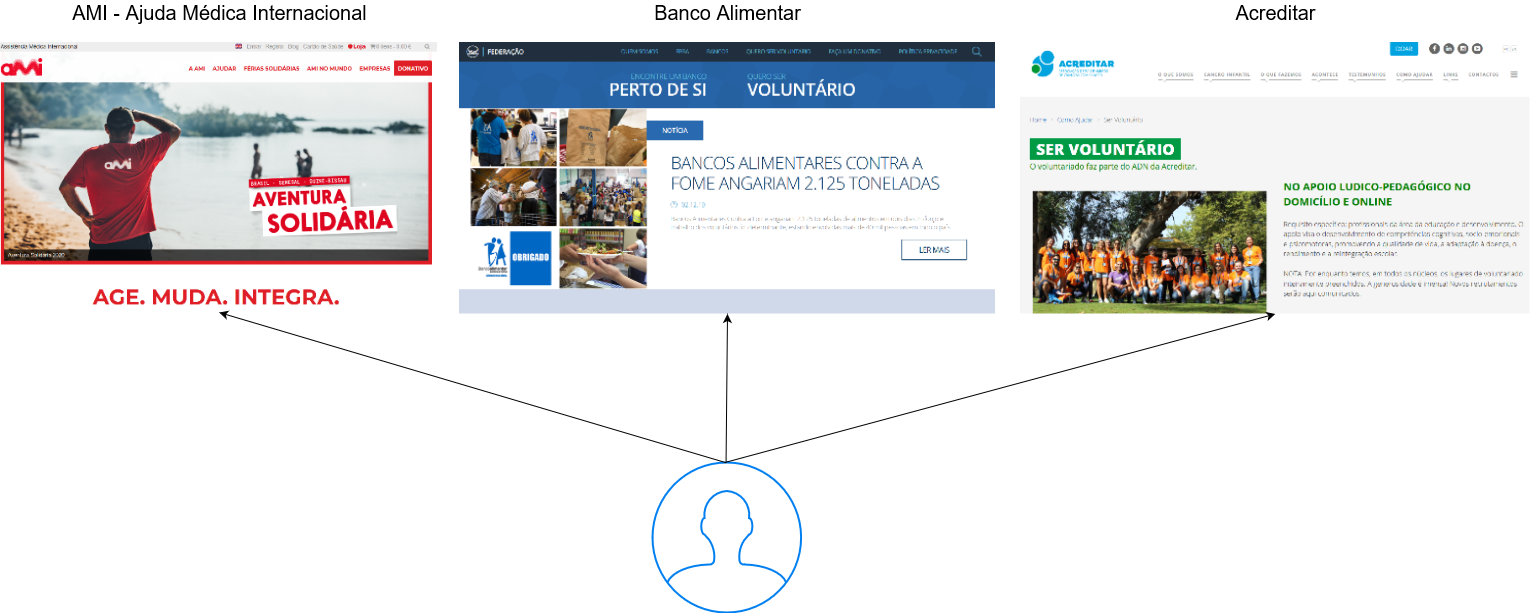
\includegraphics[scale=0.225]{services-decentralized}
	\caption{Modelo descentralizado de divulgação de voluntariado}	
\end{figure}

\newpage

O presente projeto tem como objetivo desenvolver uma rede social com foco no voluntariado. A plataforma proposta irá disponibilizar às entidades organizadoras a possibilidade de divulgar e organizar estas ações, e aos voluntários, serviços que facilitam aos mesmos manterem-se informados e participarem nas ações do seu interesse (Figura 2).

\bigskip \bigskip \bigskip

\begin{figure}[h]
	\centering
	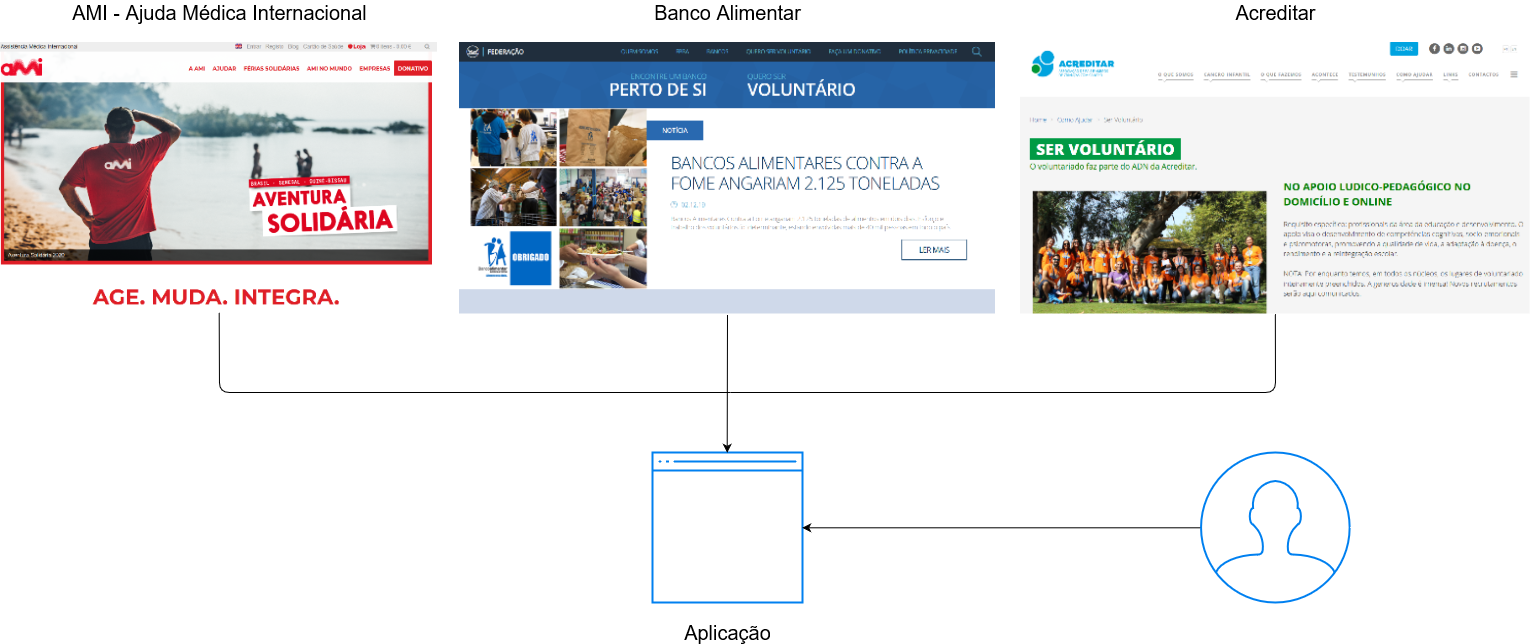
\includegraphics[scale=0.225]{services-centralized}
	\caption{Conceito do projeto}
\end{figure}

\subsection{Organização do relatório}

O restante documento encontra-se organizado em seis capítulos, descritos de seguida e pela respetiva ordem.
\begin{itemize}
	\item Formulação do problema, onde são definidos os objetivos gerais da plataforma e apresentadas outras plataformas similares. São definidos os requisitos funcionais do projeto e é escolhida a sua arquitetura;
	\item Modelo de arquitetura, capítulo responsável por discutir a arquitetura geral da plataforma e apresentar os seus módulos principais e as tecnologias utilizadas no desenvolvimento da mesma;
	\item Web API, onde é descrito o funcionamento da API usada pelas aplicações \textit{web} e móvel desenvolvidas;
	\item Mobile App, onde se aborda a implementação da aplicação cliente orientada ao voluntário;
	\item Web App, onde se apresentam detalhes relativos ao funcionamento da aplicação cliente orientada à organização;
	\item Conclusão, onde são apresentadas as conclusões tiradas após o desenvolvimento do projeto.
\end{itemize}


























\section{Modelo de Arquitetura} 
O modelo do nosso projeto(demonstrado na figura 4) é constituído por três módulos principais: uma REST API, e duas aplicações cliente: uma orientada à plataforma \textit{mobile} Android e outra desenvolvida para ser usada num \textit{browser}. \par \medskip

Tendo em conta os módulos constituintes do projeto, o desenvolvimento do mesmo seguirá o standard MEAN \textit{stack} (MongoDB, Express.js, Angular, Node.js), alternando a tecnologia utilizada para desenvolver o \textit{front-end} para React em vez de Angular (também conhecido pelo MERN \textit{stack}). Foi escolhido este \textit{standard} pelas seguintes razões:
\begin{itemize}
	\item familiaridade dos autores com algumas destas tecnologias (como Express.js e Node.js);
	\item \textit{standard} utilizado no desenvolvimento de múltiplas aplicações, o que leva a uma grande quantidade de recursos;
	\item todas estas tecnologias têm em comum características que as tornam apelativas de usar conjuntamente, como por exemplo o fact da utilização de JSON ser transversal entre todas;
	\item todas as ferramentas associadas a este modelo de desenvolvimento são \textit{open-source}.
\end{itemize}

\begin{figure}[h]
	\centering
	
\includegraphics[scale=.25]{mern}
	\caption{Tecnologias do \textit{standard} MERN}
\end{figure}

Relativamente à API, esta estabelecerá endpoints onde será possível executar pedidos HTTPS de maneira a suportar autenticação e operações na infraestrutura (criação de perfil, “seguimento” de organização, inscrição em ação de voluntariado, etc.), constituindo o \textit{back-end} do projeto.
\par \medskip

Relativamente ao \textit{front-end}, serão desenvolvidas 2 aplicações cliente: 
\begin{itemize}
	\item um cliente \textit{mobile}, para a plataforma Android, usado pelos voluntários. Nesta interface será possível efetuar por parte do utilizador as operações de uso da plataforma usuais: criação de um perfil, visionamento de um \textit{feed} de \textit{posts} efetuados pelas organizações seguidas, entre outras;
	\item um cliente \textit{browser}. Esta aplicação é direcionada às organizações e terá a finalidade de permitir às mesmas realizar \textit{posts}, criar e gerir ações de voluntariado, etc.;
\end{itemize}

\begin{figure}[h]
	\centering
	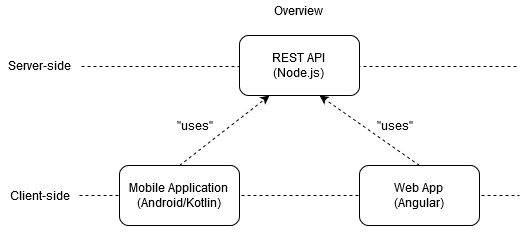
\includegraphics[scale=.8]{architecture}
	\caption{Modelo de arquitetura}
\end{figure}


\subsection{REST API}
A REST API, também definida como primeira fase do projeto, constituirá o \textit{server-side} do mesmo. É pretendido que este módulo seja completamente independente dos outros, tendo como responsabilidade trabalhar como fonte de dados para os outros componentes (client-side). \par \medskip 

A tecnologia utilizada para desenvolver este componente será Node.js em conjunto com vários package do NPM (node package manager), como o Express e o Passport. Esta escolha foi justificada por múltiplas razões:
\begin{itemize}
	\item domínio dos autores na linguagem Javascript e em vários módulos do NPM;
	\item popularidade da ferramenta, algo que simplifica o processo de desenvolvimento do componente devido à grande quantidade de recursos sobre a mesma;
	\item existência de suporte neste meio de execução de ferramentas para auxiliar o acesso à base de dados escolhida.
\end{itemize}
\par \medskip

O servidor irá ser também responsável por hospedar a base de dados, que irá funcionar no motor MongoDB. A escolha deste serviço foi efetuada devido à fácil integração do mesmo com Node.js e devido ao facto deste ter um modelo de dados baseado em documentos JSON, algo que simplifica a inserção e pesquisa sobre os mesmos.
\par \medskip

\subsection{Aplicação \textit{Mobile}}
A aplicação \textit{mobile} será desenvolvida para a plataforma Android em Kotlin. A mesma irá seguir os princípios definidos pelo Android Jetpack, que disponibiliza ferramentas e bibliotecas cujas auxiliam o desenvolvimento da aplicação. As razões que levaram a esta decisão foram:
\begin{itemize}
	\item familiaridade dos autores com esta linguagem de programação e ferramentas(Android Jetpack);
	\item a nível de quota de mercado dos sistemas operativos de dispositivos móveis, o Android é o mais prevalente;
	\item atualmente, o Kotlin é a linguagem oficial para desenvolvimento de aplicações móveis para Android.
\end{itemize}

\subsection{Aplicação \textit{Web}}
A aplicação \textit{web} será desenvolvida em React. Esta tecnologia foi escolhida devido a:

\begin{itemize}
	\item familiaridade dos autores com esta ferramenta;
	\item quota de mercado (relativamente às frameworks de Javascript utilizadas para o desenvolvimento de aplicações \textit{web}) significativa, sendo atualmente a tecnologia mais usada;
	\item integração com as outras ferramentas do projeto.
\end{itemize}

\subsection{Tecnologias e ferramentas}
As seguintes tecnologias irão ser utilizadas durante o desenvolvimento do projeto:
\begin{itemize}
	\item \textbf{Javascript}: Principal linguagem para programação client-side em browsers; Esta é tipicamente utilizada em conjunto com ferramentas como o HTML e CSS para implementar a funcionalidade de uma página web;
	\item \textbf{Node.js}: Interpretador e ambiente de execução para Javascript normalmente utilizado para executar código sem ser num cliente browser;
	\item \textbf{NPM}: package manager do Javascript/Node.js;
	\item \textbf{Express}: web framework para Node.js. Auxilia o processo de routing e definição de endpoints, encapsulando aspetos do HTTP, para tornar mais fácil o desenvolvimento de \textit{Web} APIs;
	\item \textbf{Passport}: Middleware de autenticação usado em conjunto com o Express para simplificar o processo de autenticação e gestão de sessões de utilizadores;
	\item \textbf{MongoDB}: Base de dados noSQL baseada em documentos JSON. Tipicamente integrada com Javascript devido à natureza dos seus documentos;
	\item \textbf{Android}: Sistema operativo open source para dispositivos móveis desenvolvido pela Google. Atualmente, cerca de 75\% dos dispositivos móveis usam este SO;
	\item \textbf{Kotlin}: Linguagem de programação desenvolvida pela JetBrains que compila para a JVM. Atualmente, o Kotlin é a linguagem oficial do Android;
	\item \textbf{Android Jetpack}: Conjunto de ferramentas e bibliotecas as quais auxiliam a implementação e desenvolvimento de software para o sistema operativo móvel Android;
	\item \textbf{React}: Biblioteca \textit{open-source} de Javascript usada para desenvolver a UI de aplicações.
\end{itemize}

\begin{frame}{ }
	
\centering {\Huge Demonstração}

\end{frame}

\begin{frame}{Trabalho Futuro}
	
\vspace*{-3em}
	
\begin{itemize}
	\item Aprimoramento de código desenvolvido e re-elaboração de testes unitários;
	\item adição de novas funcionalidades, como por exemplo, comentários em \textit{posts}, voluntários participantes em eventos e \textit{curriculum vitae} de voluntariado;
	\item integração de registo e autenticação usando contas de outras plataformas (através de OAuth 2.0).
\end{itemize}

\end{frame}

\end{document}